
\subparagraph{Potenziale vettore di una spira a grande distanza}
Si ricorda l'espressione del vettore potenziale
$$
\vec{A}(p) = \frac{\mu_0}{4\pi}\hat{m}\times\frac{\vec{e}_r}{r_p^2} = \frac{\mu_0}{4\pi}\vec{m}\times\frac{\vec{r}_p}{r_p^3} = -\frac{\mu_0}{4\pi}\vec{m}\times\nabla_p \left(\frac{1}{r_p} \right)
$$
È quindi possibile calcolare il campo $\vec{B}$ effettuando il rotore di $\vec{A}$
$$
\vec{B}(p) = \nabla\times\vec{A} = -\frac{\mu_0}{4\pi}\nabla_p\times\left(\vec{m}\times\nabla_p\left(\frac{1}{r_p}\right)\right)
$$
Identità vettoriale: $\nabla\times(f\vec{v}) = f\nabla\times\vec{v} + \nabla f \times \vec{v}$
$$
f = \frac{1}{r_p} \qquad \vec{v}=\vec{m}
$$
quindi
$$
\nabla\times\left(\frac{\vec{m}}{r_p}\right) = \frac{1}{r_p}\nabla\times\vec{m} + \nabla\left(\frac{1}{r_p}\right)\times \vec{m} = \frac{1}{r_p}\nabla\times\vec{m} - \vec{m}\times\nabla\left(\frac{1}{r_p}\right)
$$
L'ultimo termine può essere sostituito nell'espressione del campo ma il rotore rispetto
a $p$ del rotore di $\vec{m}$ è nullo quindi
$$
\vec{B}(p) = \frac{\mu_0}{4\pi} \nabla_p\times\nabla_p\times\left(\frac{\vec{m}}{r_p}\right)
$$
ma il rotore del rotore è il gradiente della divergenza meno il laplaciano vettore
$$
\vec{B}(p) = \frac{\mu_0}{4\pi} \left[\nabla\left(\nabla\cdot\left(\frac{\vec{m}}{r_p}\right)\right) - \cancel{\nabla^2\left(\frac{\vec{m}}{r_p}\right)}\right]
$$
Il laplaciano di $\frac{\vec{m}}{r_p}$ è nullo in quanto il momento magnetico $\vec{m}$ è 
costante come il potenziale di una carica puntiforme
$$
\vec{B}(p) = \frac{\mu_0}{4\pi}\nabla\left(\nabla\cdot\left(\frac{\vec{m}}{r_p}\right)\right) = \frac{\mu_0}{4\pi}\nabla\left(\vec{m}\cdot\nabla\left(\frac{1}{r_p}\right)\right)
$$
l'espressione tra parentesi può essere nominata $\psi$, un caso in cui il campo magnetico
può essere espresso mediante un potenziale magnetico scalare, dato che $\psi$ è una funzione 
scalare.
$$
\psi(p) = \frac{\mu_0}{4\pi}\vec{m}\cdot\nabla\left(\frac{1}{r_p}\right) = -\frac{\mu_0}{4\pi}\vec{m}\cdot \frac{\vec{r_p}}{r_p^3}
$$
Così come il potenziale di un dipolo elettrico era
$$
V(p) = \frac{1}{4\pi\varepsilon_0} \vec{p}\cdot\frac{\vec{r}_p}{r_p^3}
$$
Ciò significa che a meno di costanti e unità di misura, a grande distanza le linee di
campo magnetico prodotte da una spira circolare percorsa da corrente sono identiche alle
linee di campo elettrico prodotte da un dipolo.
\newpage
\subsection{Coefficienti di auto e mutua induzione per circuiti quasi-filiformi}
Siano presenti una serie di spire attraversate da corrente, si associano delle superfici
di orlo ad ogni linea orientate.
\begin{figure}[H]
\centering
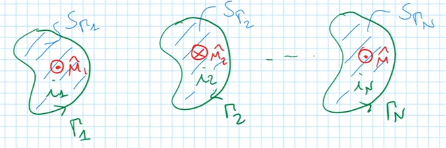
\includegraphics[width = 0.4\linewidth]{circuiti_auto_mutua_induzione}
\end{figure}
Per calcolare il campo si usa il PSE, il flusso attraverso la superficie $k$ si calcola
con 
$$
\Phi_k = \iint_{S_{\Gamma_k}}\vec{B}\cdot\hat{n}_k dS
$$
Il campo totale si può trovare con il potenziale vettore generato dalle spire
$$
\vec{A}(p) = \frac{\mu_0}{4\pi}\oint_{\Gamma_1} \frac{i_1\hat{t}_1(p')}{|\vec{r}_p - \vec{r}_{p'}|}dl_1 + ... + \frac{\mu_0}{4\pi}\oint_{\Gamma_N} \frac{i_N\hat{t}_n(p')}{|\vec{r}_p-\vec{r}_{p'}|}dl_N
$$
Sostituendo
$$
\Phi_k = \iint_{S_{\Gamma_k}} \nabla\times\vec{A}\cdot\hat{n}dS \stackrel{\text{T. di Stokes}}{=} \oint_{\Gamma_k}\vec{A}\cdot\hat{t}_kdl_k
$$
$$
\Phi_k = \oint_{\Gamma_k} \left[\frac{\mu_0}{4\pi} \oint_{\Gamma_1} \frac{i_1\hat{t}_1(p')}{|\vec{r}_p - \vec{r}_{p'}|}dl_1 + ... + \frac{\mu_0}{4\pi}\oint_{\Gamma_N} \frac{i_N\hat{t}_N(p')}{|\vec{r}_p - \vec{r}_{p'}|}dl_N \right]\cdot \hat{t}_k(p) dl_k
$$
Ma $t_k(p)$ non dipende da $p'$ si può portare all'interno degli integrali mentre
le correnti sono costanti e possono invece essere portate fuori
$$
\Phi_k = \sum_{j=i}^N \left(\frac{\mu_0}{4\pi} \oint_{\Gamma_k}\oint_{\Gamma_j} \frac{\hat{t}_j(p')\cdot\hat{t}_k(p)}{|\vec{r}_p-\vec{r}_{p'}|} dl_j dl_k \right)i_j
$$
Il termine tra parentesi è tutto sommato uno scalare che dipende da due indici quindi lo 
riassumiamo con $L_{kj}$
$$
\Phi_k = \sum_{j=i}^N L_{kj} i_j
$$
Il coefficiente prende nomi differenti
$$
\begin{cases}
L_{kk} & \text{Coefficiente di autoinduzione della spira } k\\
L_{kj} & \text{Coefficiente di mutua induzione tra la spira } k \text{ e } j
\end{cases}
$$
Combinando tutti i coefficienti si ottiene una matrice $N\times N$ di coefficienti definiti
$$
L_{kj} = \left.\frac{\Phi_k}{i_j}\right|_{i_S = 0,\ S\neq j}
$$
Il flusso che l'avvolgimento $j$ produrrebbe da solo concatenato con $k$ se la corrente
$i_j$ agisse da sola con tutte le altre uguali a zero ossia l'effetto nel circuito $k$
della causa nel circuito $j$.

Una proprietà analoga si ritrova nei doppi bipoli resistivi che godono della proprietà di
reciprocità per il \href{https://it.wikipedia.org/wiki/Teorema_di_Tellegen}{teorema di Tellegen} ossia che il rapporto tra causa ed effetto tra due circuiti diversi è uguale.

Si vede dunque che $L_{kj} = L_{jk}$ perché negli integrali è presente il prodotto
scalare tra i versori $\hat{t}_j$ e $\hat{t}_k$ che gode della proprietà commutativa,
inoltre si invertirebbero tutti gli indici degli integrali.

Il coefficiente di autoinduzione $L_{kk}$ è intrinsecamente positivo dato che 
l'orientamento del campo 
è concorde con l'orientamento della curva se quest'ultimo rispetta il verso della corrente.
Ciò non è sempre vero se gli avvolgimenti sono diversi dato gli orientamenti delle 
linee sono indipendenti tra loro.

\textbf{Osservazione:} il circuito non può essere realmente filiforme perché avrebbe al suo
interno un campo che divergerebbe.
40:30
